\documentclass{article}
\usepackage{graphicx} % Required for inserting images
\usepackage[left=2cm,right=2cm,top=2cm,bottom=2cm]{geometry} 
\usepackage{setspace} 
\onehalfspacing
\usepackage{float}
\usepackage{fancyhdr}
\usepackage{booktabs}
\usepackage{array}
\usepackage{longtable}
\usepackage{geometry}
\usepackage{amsmath}
\usepackage{amsfonts}
\usepackage{mathrsfs}

\fancyhead[LO]{\small{\textit{Time Series Analysis: Assignment 2}}}

\title{\textbf{Time Series Analysis - Assignment 2}\\Econometrics and Data Science}
\author{
    Geesink, T. \\
    \texttt{14124165}
    }
    
\date{March 2026}

\begin{document}
    \pagestyle{fancy}

\includegraphics[scale=0.2]{logo.jpg}
\begingroup
{\let\newpage\relax\maketitle}
\maketitle
\endgroup 

\clearpage

\section*{Part 1}
This part considers the GARCH($m, s$) model, that is,

\begin{align*}
y_t &= \mu + \varepsilon_t \\
\varepsilon_t &= \sigma_t \nu_t \\
\sigma_t^2 &= \alpha_0 + \sum_{i=1}^{m} \alpha_i \varepsilon_{t-i}^2 + \sum_{j=1}^{s} \beta_j \sigma_{t-j}^2,
\end{align*}
where $\nu_t \sim \text{i.i.d. } \mathcal{N}(0, 1)$. The $h$-step-ahead forecast for the conditional variance is defined by: $\hat{\sigma}_{n+h}^2 = \mathbb{E}[\sigma_{n+h}^2 | \mathcal{F}_n]$. Here $\mathcal{F}_n$ contains all information (conditional variances and residuals) up to time $n$.

\begin{enumerate}
    \item[(a)] Show that the ARCH($m$) model for the conditional variance can be rewritten as an AR($m$) model for the squared residuals $\{\varepsilon_t^2\}$. \newline \newline
    A: 
    \begin{align}
    \sigma_t^2 &= E(\varepsilon_t^2 | \mathcal{F}_{t-1}) \\ &= \alpha_0 + \sum_{i=1}^m \alpha_i \varepsilon_{t-i}^2 \\
    \sigma_t^2 + \varepsilon_t^2 &= \alpha_0 + \varepsilon_t^2 + \sum_{i=1}^m \alpha_i \varepsilon_{t-i}^2 \\
    \Leftrightarrow \varepsilon_t^2 &= \alpha_0 + \sum_{i=1}^m \alpha_i \varepsilon_{t-i}^2 + (\varepsilon_t^2 - \sigma_t^2) \\
    \Leftrightarrow \varepsilon_t^2 &= \alpha_0 + \sum_{i=1}^m \alpha_i \varepsilon_{t-i}^2 + \xi_t
    \end{align}
    where $\xi_t = \varepsilon_t^2 - \sigma_t^2$ is WN, as $E(\xi_t) = 0$ and $E(\xi_t \xi_{t-h}) = 0 \quad \forall h \neq 0$.
    Thus, $\{\varepsilon_t^2\}$ follows an AR($M$) process
    \newpage
    \item[(b)] Suppose you have an observed time series $\{y_t\}_{t=1}^T$. Assume that $\mu = 0$. Using the error decomposition of Q1c in Assignment 1, derive the likelihood of the GARCH($m, s$) model. Additionally, derive the first-order conditions. \newline \newline
    A:
    \begin{align}
    \mu = 0 \Rightarrow y_t = \varepsilon_t = \sigma_t \nu_t \sim \mathcal{N}(0, \sigma_t^2) \\
    \quad y_t^2 | \mathcal{F}_{t-1} = \alpha_0 + \sum_{i=1}^m \alpha_i \varepsilon_{t-i}^2 + \xi_t \\
    \text{So} \quad f(y_t | \mathcal{F}_{t-1}) = \frac{1}{\sqrt{2\pi\sigma_t^2}} e^{ -\left(\frac{y_t}{2\sigma_t} \right)^2}
    \end{align}
    \begin{align}
    L(\alpha_0, \alpha_1, \dots, \alpha_m, \beta_1, \dots, \beta_s) &= f(y_t, y_{t-1}, \dots, y_1) = f(y_t | \mathcal{F}_{t-1}) \cdots f(y_2 | y_1) f(y_1) \\
    &= \prod_{j=1}^t \frac{1}{\sqrt{2\pi\sigma_j^2}} \exp \left( -\sum_{i=1}^t \frac{y_i^2}{2\sigma_i^2} \right) = \prod_{j=1}^t \frac{1}{\sqrt{2\pi\sigma_j^2}} \exp \left( -\sum_{i=1}^t \frac{\varepsilon_i^2}{2\sigma_i^2} \right) \\
    \Rightarrow l(\alpha, \beta) &= \log L(\alpha, \beta) \\
    &= -\frac{t}{2} \log(2\pi) - \frac{1}{2} \sum_{j=1}^t \log(\sigma_j^2) - \frac{1}{2} \sum_{j=1}^t \frac{\varepsilon_j^2}{\sigma_j^2}
    \end{align}
    \begin{align}
    \Rightarrow f.o.c.'s : \quad \frac{\partial l(\alpha, \beta)}{\partial \alpha_0} &= -\frac{1}{2} \sum_{j=1}^t \frac{1}{\sigma_j^2} - \frac{\varepsilon_j^2}{\sigma_j^4} = 0 \\
    \frac{\partial l(\alpha, \beta)}{\partial \alpha_i} &= 0 \quad \text{for} \quad i = 1, \dots, m \\
    \frac{\partial l(\alpha, \beta)}{\partial \beta_j} &= 0 \quad \text{for} \quad j = 1, \dots, s
    \end{align}

    \newpage
    \item[(c)] Which restrictions on $\alpha_0, \alpha_1, \dots, \alpha_m$ and $\beta_1, \dots, \beta_s$ are needed to ensure positivity for the conditional variance? And under which restrictions does the conditional variance satisfy stationarity? \newline\newline
    A:
    \begin{align}
    \alpha_{0} \geq 0, \ \alpha_{i} \geq 0 \quad \forall i=1, \dots, m, \quad \beta_{j} \geq 0 \quad \forall j=1, \dots, s
    \end{align}
    
    $\alpha_{0} > 0$ can also be taken, such that the conditional variance is per definition positive (in combination with the other restrictions). For stationarity, we need
    
    \begin{align}
    \sum_{i=1}^{m} \alpha_{i} + \sum_{j=1}^{s} \beta_{j} < 1
    \end{align}
    
    to ensure that the conditional variance does not 'explode' (grow indefinitely), and that the process has no unit roots. Regarding stationarity, we do not need to restrict $\alpha_{0}$ as its impact on the conditional variance is time invariant.
\end{enumerate}

\newpage
\section*{Part 2}
In this part, you are asked to download data yourself again and make estimates and forecasts, assuming a GARCH($1,1$) model for the conditional variance.
\begin{enumerate}
    \item [(a)] Download daily data from the website of Yahoo Finance for the Amsterdam Exchange Index (ticker: ˆAEX) from January 1, 2010, up to and including December 31, 2025. Save as a CSV file and enable your script to read the data. Use the adjusted closing prices as our time series. You are allowed to use a package for downloading the data. \newline \newline
    A: See R code 'Part 2a'
    \item [(b)] Calculate the daily log-returns and plot the log-returns and the squared log-returns over time. What can you say about the series’ volatility based on this plot (is volatility constant over time or is there heteroskedasticy of some sort)?
    \begin{figure}
    \centering
    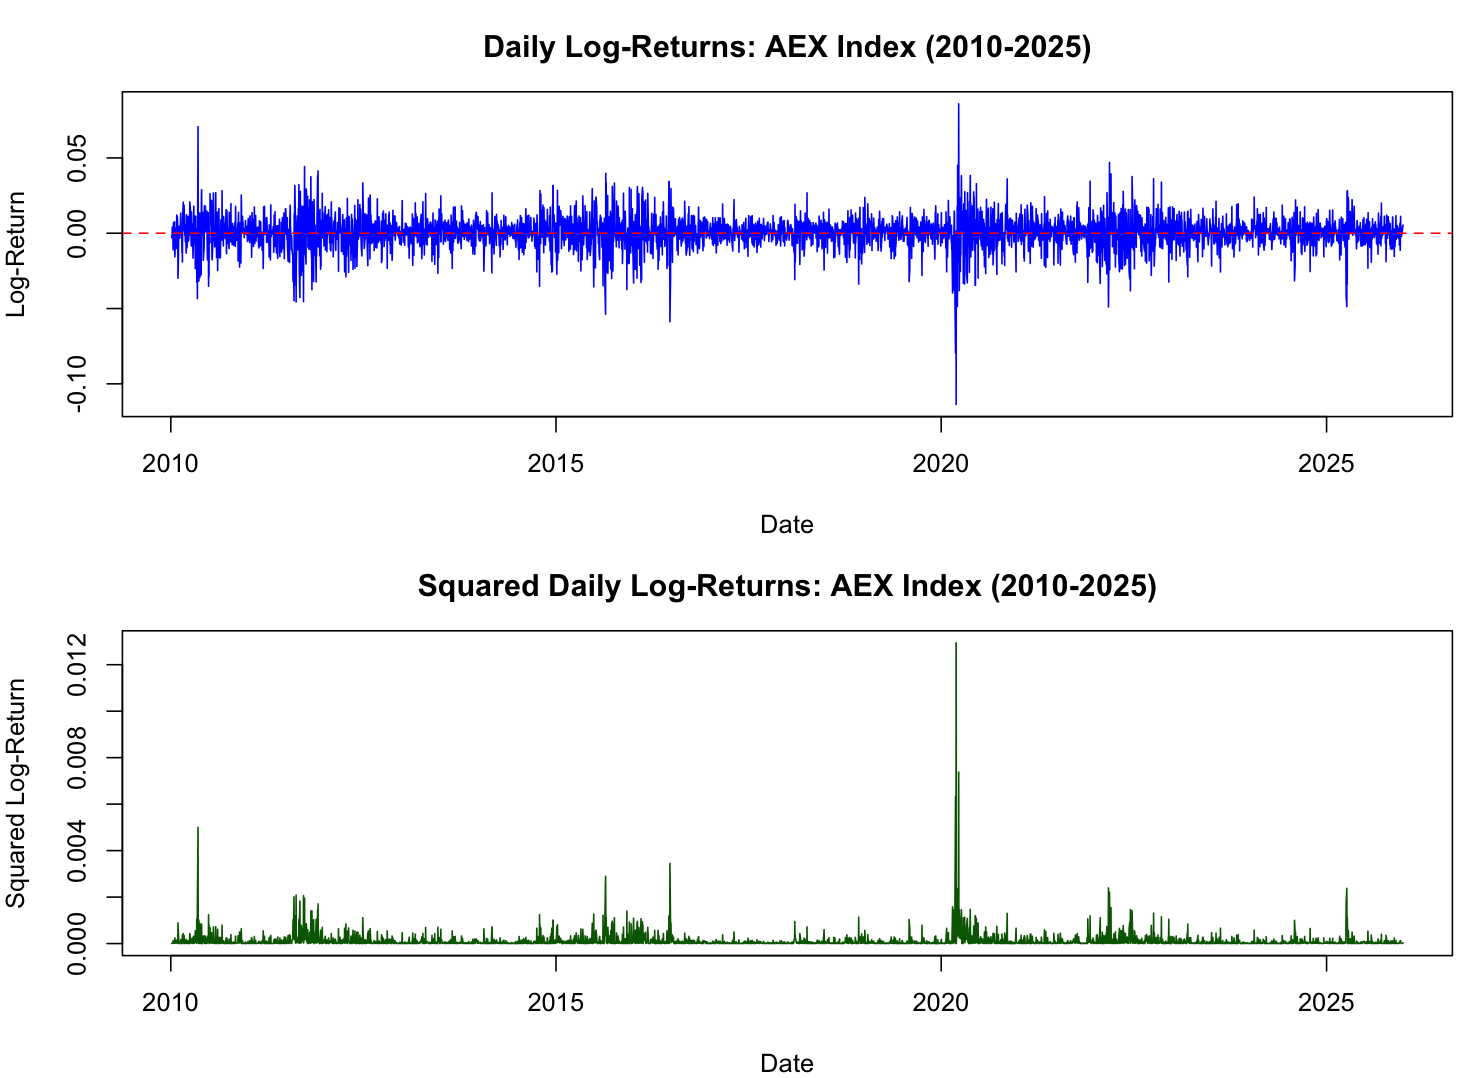
\includegraphics[width=0.8\linewidth]{Assignment 2 Part 2b.png}
    \caption{(b)}
    \end{figure}
    \newline \newline
    A: The plots clearly demonstrate that the volatility is not constant over time, hence there is heteroskedasticity. Large changes tend to be followed by large changes, and small changes tend to be followed by small changes. we see distinct spikes in the squared returns, confirming that the variance is clustering and changing over time.

\end{enumerate}
\newpage
The last 20 data points are not used for estimating, but for comparing to our forecasts later. Split your data points into a set containing these last 20 values and an estimation set, containing all other data points.
\begin{enumerate}
    \item [(c)] Estimate the model using the Maximum Likelihood, assuming that $\mu = 0$. As starting values, you may use the sample variance of the log-returns over the whole estimation sample as the first conditional variance and you may assume $\varepsilon_t = 0$ as starting value for the error term. Interpret the results. What do the estimated coefficients imply for the conditional variance based on information of earlier returns? \newline \newline
    A:$$\sigma_t^2 = \alpha_0 + \alpha_1 \varepsilon_{t-1}^2 + \beta_1 \sigma_{t-1}^2$$
    
    $\alpha_0 =$ 5e-06: As expected for daily log-returns, this value is extremely small so the conditional variance doesn't drop to zero. 
    
    $\alpha_1 = 0.109396...$: This coefficient measures the reaction of the conditional variance to new information (squared error from the previous day, $\varepsilon_{t-1}^2$). The value of approximately $0.11$ means that the variance is sensitive to yesterday's information. This parameter is responsible for the "spikiness" we see in the squared returns plot. 
    
    $\beta_1 = 0.834404...$: Measures how much of yesterday's variance ($\sigma_{t-1}^2$) carries over to today. A high value of approximately $0.83$ indicates strong volatility clustering; if the market was highly volatile yesterday, it is strongly predicted to remain volatile today.
    
    $\alpha_1 + \beta_1 = 0.943801...$: $\alpha + \beta < 1$ means the conditional variance will eventually go to its mean rather than exploding to infinity. Because the sum is very close to $1$, the volatility is highly persistent. Shocks decay slowly. It will take a significant amount of time for the conditional variance to go back down to its long-run unconditional average.
\newpage
With the model estimated, the logical next step is to evaluate its predictive power on your holdout set. Would you like to walk through how to calculate the 1-step to 20-step ahead forecasts for the conditional variance to compare with those last 20 data points?
    \item[(d)] Test the model assumption of normally distributed errors. In case this assumption is rejected, what other distribution for the error terms can you think of? \newline \newline
    \begin{figure}
        \centering
        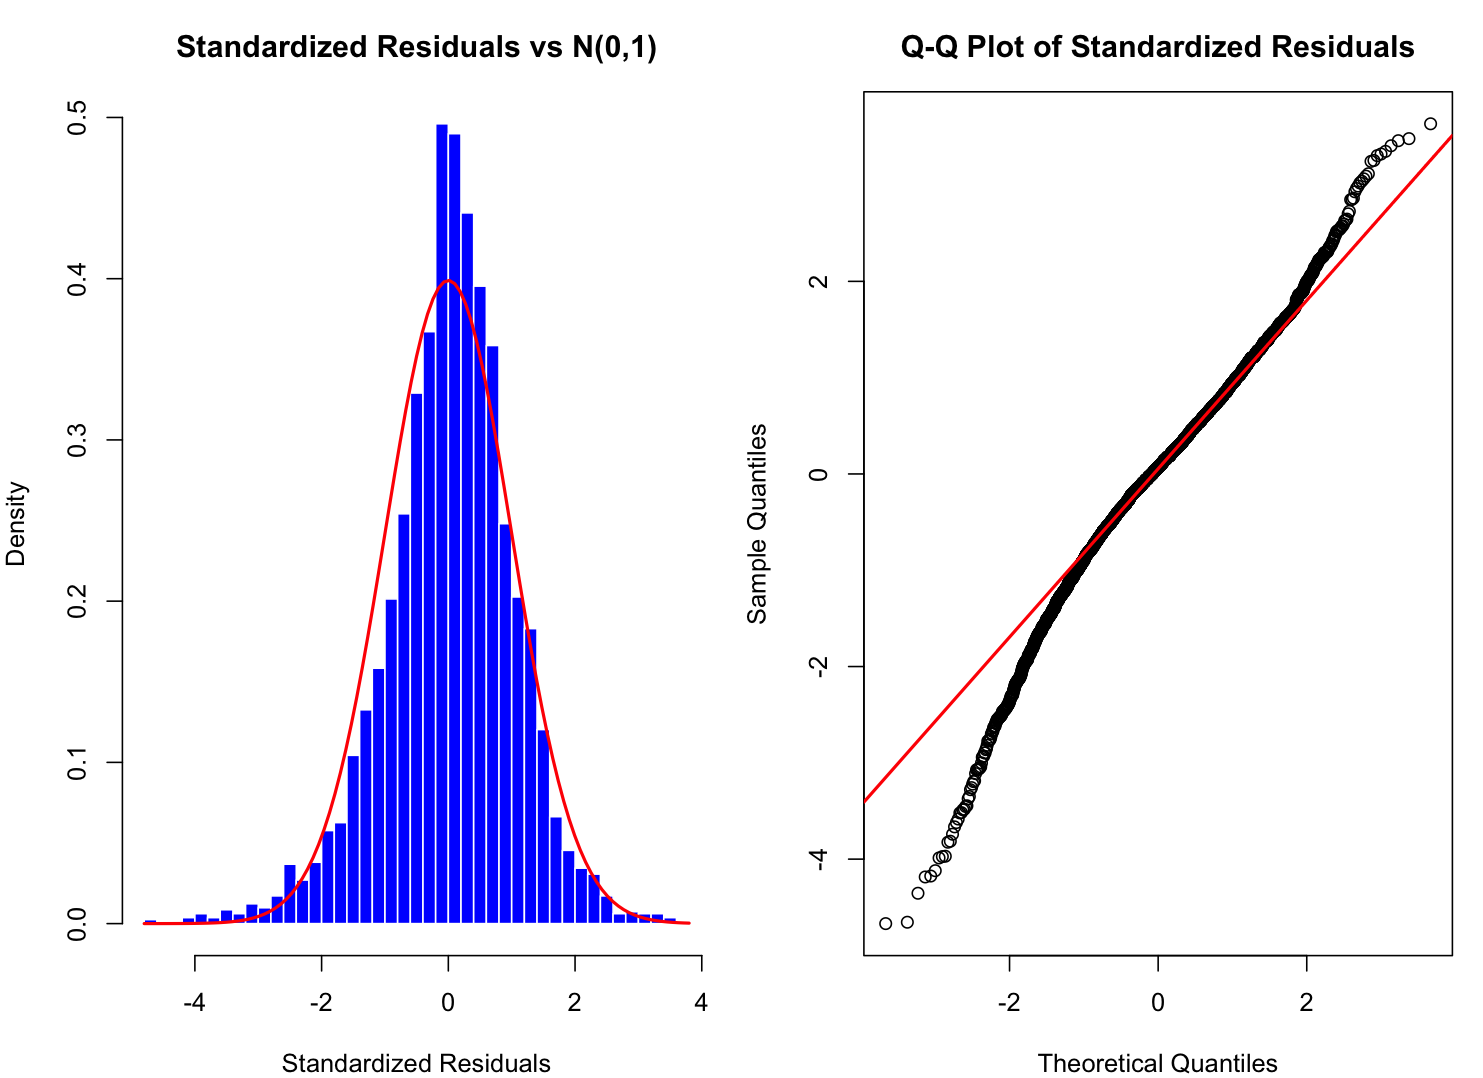
\includegraphics[width=0.8\linewidth]{Assignment 2 part 2d.png}
        \caption{(d)}
    \end{figure}
    A: Jarque-Bera Test Results (X-squared = 419.86, df = 2, p-value < 2.2e-16): We reject the null hypothesis. large positive or negative shocks are still happening more frequently than a normal distribution would predict. Since the assumption of normal errors ($\varepsilon_t \sim N(0,1)$) is violated, the Skewed Student's t-Distribution would be an appropriate option since the returns often have negative skewness (tends to crash faster than they rise).
    \newpage
    \item[(e)] Now, estimate the model using the “rugarch” package in R (so now you are allowed to use functions defined in R to estimate the GARCH model), or a similar module in Python. Compare these results to the results from MLE obtained in (c). Also, plot the fitted conditional variances and the squared residuals over time. Comment on the quality of the fit. \newline \newline
    \begin{figure}
        \centering
        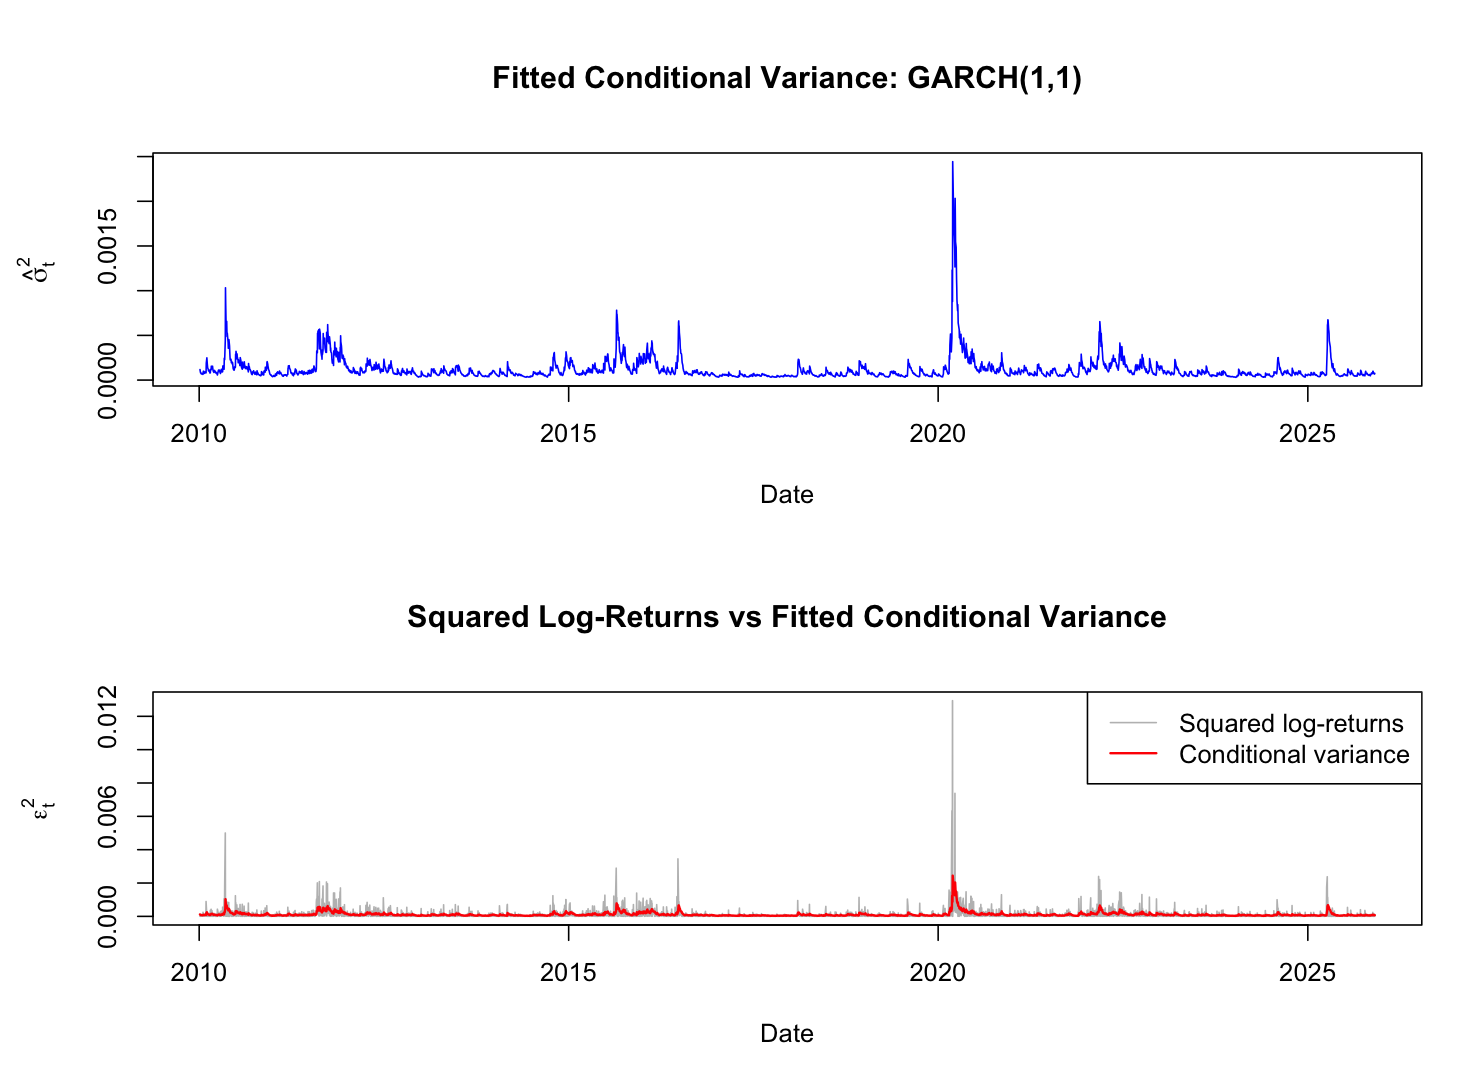
\includegraphics[width=0.8\linewidth]{Assignment 2 Part 2e.png}
        \caption{(e)}
    \end{figure}
    A: The estimates from the MLE and the rugarch package are very close, which confirms that the manual implementation is functioning correctly. 
    
    $\hat{\beta}_1$: The memory of the variance is almost identical between the two methods ($0.8344$ vs $0.8336$). 
    
    $\hat{\alpha}_1$: The rugarch package estimates a slightly higher sensitivity to recent shocks ($0.1319$ vs $0.1094$). 
    
    $\hat{\alpha}_1 + \hat{\beta}_1$: Because of the higher $\hat{\alpha}_1$, the rugarch model suggests slightly higher volatility persistence ($0.965$ vs $0.944$). Based on the plots, the GARCH($1,1$) model provides a very solid fit for capturing the volatility dynamics of the AEX index. In the bottom plot, the fitted conditional variance, $\hat{\sigma}_t^2$ acts highly responsive for the grey spikes (squared log-returns, $\varepsilon_t^2$). When the squared returns cluster, the conditional variance appropriately ramps up. When the grey spikes are small and sparse, the red line correctly settles back down toward the unconditional baseline. The red line spikes significantly during the 2020 crash, but it does not stretch all the way to the absolute peak of the tallest grey spike. 
    
    We can see the high persistence ($\alpha + \beta \approx 0.965$) in the top plot. After big spikes (like in 2011 and 2020), the blue line takes a considerable amount of time to decay back to its lowest levels, reflecting the long memory typical of financial volatility. While this baseline fit is strong, the GARCH($1,1$) model with normal errors is symmetric and treats negative and positive shocks identically, which we know from the previous Jarque-Bera test might leave some tail behavior unexplained.
    \newpage
    \item[(f)] Use the estimated parameters from (c) to make forecasts for the conditional variance up to 20 days forward. Note: for constructing the forecasts, you must write your own code again! Plot the forecasts and use them in your report. Also plot the actual squared returns and compare them to the conditional variance forecasts. \newline \newline
    \begin{figure}
        \centering
        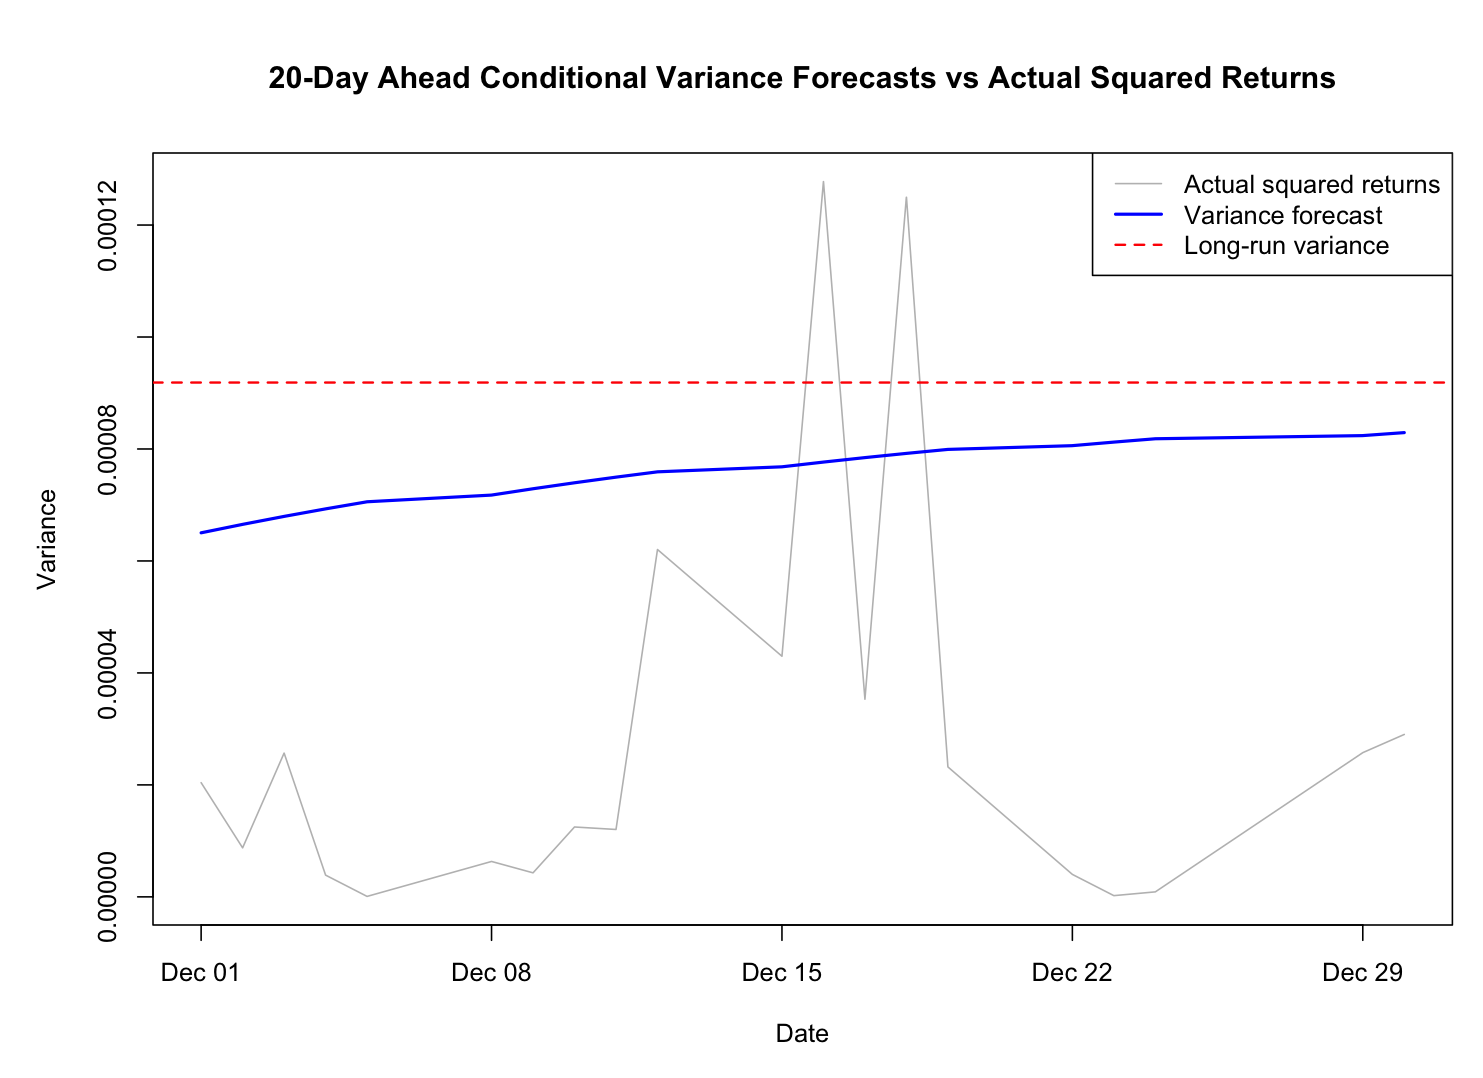
\includegraphics[width=0.8\linewidth]{Assignment 2 Part 2f.png}
        \caption{Enter Caption}
        \label{fig:placeholder}
    \end{figure}
    A: The solid blue line starts at a level below the red dashed line and gradually curves upwards. The red dashed line represents the unconditional, long-run variance (9.187e-05). Because the conditional variance at the end of the estimation sample was lower than the historical average, the model correctly predicts that volatility will slowly rise back toward its long-term baseline. 
    
    The slope of that blue line is dictated by the persistence parameter ($\hat{\alpha}_1 + \hat{\beta}_1$). As estimated earlier, is approximately 0.944. Because this value is close to 1, the "memory" of the recent low volatility takes a long time to fade. Consequently, the blue line climbs very gradually, showing that it will take many more than 20 days to fully reach the red dashed line. 
    
    The blue forecast line represents the expected variance based on information available at time $T$. The grey line represents the actual realized squared returns, which consist of the expected variance plus the random daily shock ($\varepsilon_{T+k}^2$). Therefore, the grey line is naturally chaotic and noisy. For the first part of December, the actual returns are relatively quiet, sitting below the forecast line. However, around mid-December, the market experienced massive, sudden shocks, sending the actual squared returns spiking far above both the forecasted variance and the long-run variance.
\end{enumerate}

\newpage
\section*{Part 3}
\begin{enumerate}
    \item [(a)] Download daily data from the website of Yahoo Finance for the 10-year Treasury Yield (ticker: ˆ TNX) from January 1, 2010, up to and including December 31, 2025. Save as a CSV file and enable your script to read the data. Use the adjusted closing prices as our time series. Note that the data may contain days without a value (non-trading days). Make sure you remove these empty entries. Calculate the daily log-returns.
    \newline \newline
    A: See R code 'Part 3a'
    \item[(b)] Use the full sample to estimate five AR(p) models, namely for $p = 1,2,3,4,5$ and report the log likelihood, AIC and BIC based on the full sample for each of the five AR specifications. Explain the difference between the in-sample log-likelihoods and AICs. Also report the optimal lag order based on the AIC.
    \newline \newline
    A: As we add more parameters, the model becomes more flexible and can capture more of the specific variations in the training sample. So, the log-likelihood will increase (from $8722.67$ to $8749.42$). However, a complex model will fit the noise in the sample rather than the true underlying data-generating process, resulting in poor out-of-sample forecasts. To counter the overfitting problem, the AIC penalizes the addition of extra parameters. It is generally defined as:
    $$AIC = 2k - 2\log(L)$$
    Where $k$ is the number of estimated parameters and $L$ is the maximized log-likelihood. While the fit component ($-2\log(L)$) decreases as we add lags, the penalty component ($2k$) increases. The AIC seeks the optimal balance. A lower AIC value indicates a better model.
    
    Based on the results, the optimal lag order is $p = 5$. As clearly illustrated in the plot, the AIC value strictly decreases as the number of lags increases, reaching its minimum at $-17484.83$ when $p = 5$.
    
    The BIC, which has a much stricter penalty for complexity ($\log(T)k$ instead of $2k$), agrees with this selection.
\end{enumerate}
\newpage
To compare different models, we often would like to test the out-of-sample performance, where the forecasts are compared to the actual observations. In time series it is customary to use rolling window forecasts. With this method, a subsample is used to calculate the one-step-ahead forecast. Then the subsample moves one observation forward, but remains of the same size, so the first observation in the previous subsample is dropped. Again the one-step-ahead forecast is calculated. This is repeated until the end of the full sample is reached. Note that your first forecast corresponds to the first observation after the subsample size m. Rolling the window through the data produces a sequence of $N-m$ forecasts $\hat{y}_i$ which can be compared with their actual values $f_i$ by the RMSE, defined as
$$
\text{RMSE} = \left( \frac{1}{N-m} \sum_{i=m+1}^{N} (y_i - \hat{y}_i)^2 \right)^{1/2}
$$
\begin{enumerate}
    \item [(c)] Extend your code for OLS estimation from assignment 1 and use a fixed estimation window method to obtain forecasts for the remaining log-returns, for AR($p$) models for $p= 1,2,3,4,5$. Use the window consisting of the first 750 observations to estimate the models and generate 1-step-ahead forecasts for the remaining observations. Calculate the RMSE’s and save the results for the different AR($p$) specifications. \newline \newline
    A: See R code 'Part 3c'
    
    \item[(d)] Repeat (c), but now re-estimate the models at each step. Hence, also use a rolling estimation window. At each step, use the previous 750 observations to estimate a new model and calculate the one-step-ahead forecasts, instead of estimating the model only once (based on the first 750 observations) and using this model to obtain all rolling window forecasts. \newline \newline
    A: See R code 'Part 3d'
\end{enumerate}
Another variation on the rolling window method is the expanding window method, in which the window length expands at each step. So as opposed to in the rolling window method, no observations are dropped and the estimation subsample becomes larger each step. For example, the first step is to estimate the model based on the first 750 observations and then use that model to make the first forecast. The next step would be to re-estimate the model based on the first 751 observations and then make the one-step-forecast based on the new estimated model. This continues until the end of the sample is reached.
\begin{enumerate}
    \item [(e)] Use the expanding window method to obtain forecasts for the log-returns, for AR($p$) models for $p = 1,2,3,4,5$. Calculate the RMSE’s and save the results for the different AR($p$) specifications. \newline \newline
    A: See R code 'Part 3e'
    \newpage
    \item [(f)] Consider the RMSE’s obtained in (c), (d) and (e) for the different AR($p$) models. Discuss results, what is the optimal AR model? Are there differences between the methods? Does the conclusion correspond to the one in (b)? \newline \newline
    A: Across all three methods, AR(1) consistently achieves the lowest RMSE, making it the preferred specification from an out-of-sample forecasting perspective. The ranking of models is identical across all methods, RMSE increases monotonically with lag order $p$.
    
    The fixed and rolling window methods produce identical RMSE values. The expanding window consistently produces lower RMSE values across all lag orders, suggesting that retaining all historical observations improves parameter precision for this particular series, consistent with a stable and stationary data generating process.
    
    The out-of-sample results contradict the in-sample findings from part (b), where both AIC and BIC selected AR($5$) as the optimal specification.
    
    For the in-sample, adding more lags always improves the log-likelihood and reduces AIC/BIC to justify their inclusion. Out-of-sample, the additional lags capture noise rather than genuine signal, leading to worse forecasts due to overfitting.
\end{enumerate}
\end{document}
